% ============================================================================
% STITCH Phase 3: a real-MPSoC case study (full results write-up)
% ----------------------------------------------------------------------------
% Companion to STITCH_EXT_v7.tex, Section 9. Self-contained: compiles on its
% own in Overleaf with the figures/ folder next to it. ASCII only, no em-dashes.
%
% Every number comes from phase3/evidence/phase3_run/PHASE3_RESULTS.md, which
% phase3/runner/analyze_phase3.py generates from the 990 metrics.json files in
% phase3/results/phase3_run/. After a new run, regenerate that file and update
% the numbers here from it; never edit a number by hand from memory.
%
% Figures (figures/, copied from phase3/evidence/phase3_run/figures/):
%   fig_p3_clean_by_condition.png, fig_p3_composition.png,
%   fig_p3_clean_by_call.png, fig_p3_v3_vs_raw_by_model.png
% ============================================================================

\documentclass[11pt]{article}

\usepackage[margin=1in]{geometry}
\usepackage{booktabs}
\usepackage{tabularx}
\usepackage{graphicx}
\usepackage{xcolor}
\usepackage{enumitem}
\usepackage{amsmath}
\usepackage{hyperref}
\hypersetup{colorlinks=true, linkcolor=blue!50!black, urlcolor=blue!50!black}
\graphicspath{{figures/}}

\title{\textbf{STITCH on a Real MPSoC}\\[4pt]
\large\textnormal{Catching Simulation-Silent Defects, Interpreting Them, and
Restoring Synthesis of a Multiprocessor Design}}
\author{Karthikeya Patana \and Yashwant Rajesh \and Aathira Sunil \and Durga Saranyu \and Sri Parameswaran \and Kamesh Chandrasekar \and Paresh Saxena \and Soumya Joshi}
\date{Phase~3 results, $990$ runs}

\begin{document}
\maketitle

\begin{abstract}
STITCH translates Verilator and Yosys output into targeted repair directives
for a language-model repair loop. Earlier phases measured it on single-module
benchmarks. This report asks what it does on real hardware: an independently
developed RISC-V MPSoC with a mesh network-on-chip, whose own reference RTL
already contains latches and a register that makes Yosys abort. We repair
$11$ defective modules ($8$ real leaves, $3$ seeded) with six local models
($3$B to $14$B) under five feedback conditions, $N{=}3$, one shared budget of
six model calls: $990$ runs. Four results stand out. (1) A simulation-only
loop signs off $62\%$ of its runs with the structural defect still present,
and all $108$ runs on defects that simulation cannot see; with STITCH the
share of signed-off defective runs falls to $1\%$. (2) Interpreted feedback
beats the same raw tool text by $14.6$ points of clean pass rate (cell-level
$95\%$ CI $+3.5$ to $+26.3$), with $23\%$ fewer model calls and tokens, and
reaches $62\%$ of runs clean after a single call. (3) Repaired leaves compose:
spliced back into the real designs, they restore top-level synthesis of the
$4$-router and $9$-router meshes and of the MPSoC, which simulation-only repair
never achieves, and every set of clean leaves produced a design at the golden
bound. (4) Escalation reaches the highest clean pass rate ($80\%$) and beats
simulation-only repair on the defects simulation does reveal ($+23.3$ points,
CI $+8.9$ to $+37.8$). An additive interpreter upgrade (v3), driven by the
design's real logs, closes the vocabulary gaps the production interpreter
showed there, without changing its behaviour anywhere else.
\end{abstract}

% ============================================================================
\section{Why a Real MPSoC}
\label{sec:why}

The single-module studies established \emph{when} STITCH's interpreter acts:
where the model produces a defect the tools can see and the interpreter can
name. They also rested on an argument they could not test: primitives compose.
A defect repaired once in a leaf definition is repaired in every instance of
it, so leaf-level repair should carry to the system. This phase tests that
argument on a design nobody wrote for this study, and asks the practical
question behind it: does STITCH catch the defects that decide whether a real
multiprocessor design can be signed off?

% ============================================================================
\section{The Substrate Already Contains the Target Defects}
\label{sec:substrate}

The design is an in-group MPSoC: a five-stage RV32 core, a network interface
(packetiser, depacketiser, asynchronous FIFOs) and a virtual-channel wormhole
mesh router, available as a $2{\times}2$ mesh ($4$ routers) and a $3{\times}3$
mesh ($9$ routers) that share $28$ of $33$ router leaf files. Only
compile-level changes were made for the open-source flow (redeclarations,
nested comments, and Vivado-style implicit trailing ports reproduced with
identical binding); no structural defect was touched.

Synthesis of the MPSoC top reports $63$ latch inferences across $12$ module
definitions and then aborts: a one-bit register tests \texttt{clr | reset}
inside an asynchronous-reset block, which Yosys cannot map. These defects are
\emph{simulation-silent}. Every latch-bearing multiplexer examined behaves
correctly on its intended inputs, and the aborting register simulates
correctly. A simulation-only repair loop has nothing to react to. Because the
top-level testbench is a weak oracle (two instructions, the network never
exercised), all top-level claims here are structural, and functional claims
rest on per-module, specification-based testbenches.

\subsection{Defects propagate with instance count; the feedback does not}

Both meshes inherit two latching register definitions ($32$ and $4$ latched
bits), each instantiated $20$ times per router (Table~\ref{tab:prop}). Yosys
reports one latch message per module \emph{definition}, so a repair loop sees
the same two messages at $N{=}4$ and $N{=}9$, while the physical damage grows
exactly with router count. The leverage of a leaf repair therefore grows with
the design.

\begin{table}[htbp]
\centering
\caption{Two leaf defects composed into the real mesh routers
($6{,}480/2{,}880 = 9/4$). Repairing three leaf definitions restores both
meshes. For the MPSoC top, repairing the eight task leaves turns the abort into
a pass; $122$ latch cells remain, all in five modules outside the repair set,
so the MPSoC bound is restored synthesisability, not a latch-free design.}
\label{tab:prop}
\small
\begin{tabularx}{\linewidth}{@{} X c c c @{}}
\toprule
 & \textbf{$2{\times}2$ mesh} & \textbf{$3{\times}3$ mesh} & \textbf{MPSoC top} \\
\midrule
Yosys latch messages (as written)      & $2$ & $2$ & $63$ \\
Latch cells, abort-causing file excluded & $2{,}880$ & $6{,}480$ & $269$ \\
Top-level synthesis, as written          & aborts & aborts & aborts \\
Top-level synthesis, task leaves golden  & pass, $0$ cells & pass, $0$ cells & pass, $122$ cells \\
\bottomrule
\end{tabularx}
\end{table}

% ============================================================================
\section{Keeping the Interpreter Robust: the v3 Layer}
\label{sec:v3}

Running the production interpreter (v2, used unchanged in every earlier phase)
on the real MPSoC logs exposed gaps that synthetic tests had not:
\begin{itemize}[leftmargin=1.2em, itemsep=0.1em]
\item \textbf{Wrong advice.} An unused \emph{clock} got the generic gating
template (\texttt{if (clk)} inside a combinational block), which builds a
clock-gated latch; a legitimately part-unused instruction bus was turned into
``gate the output on this bus''; one file holding several modules produced
advice for the wrong module.
\item \textbf{No advice.} The asynchronous-reset abort names no signal and had
no handler; a width truncation whose operand is an expression was dropped; a
loop that only Verilator reports never reached the model.
\end{itemize}

v3 is an additive layer. It imports the production interpreter unchanged,
reproduces its output byte for byte wherever no new rule applies (tests enforce
this), caps output at three directives, and adds a rule only where a real log
showed the production directive wrong or missing. Its most consequential rule
is cross-tool fusion: a Yosys latch in a level-sensitive block together with a
Verilator unused-clock warning is diagnosed as a missing clock edge rather than
as either warning alone. A live drift gate runs the interpreter on fresh tool
output before any GPU time is spent; it caught a latch-message format change
between the development toolchain (Yosys~$0.33$) and the cluster toolchain
(Yosys~$0.69$) that would otherwise have silently disabled the new rules.

% ============================================================================
\section{Experiment}
\label{sec:exp}

\textbf{Tasks.} Eleven repair tasks: the eight defective real leaves and three
seeded RISC-V/NoC modules for classes absent from the reference
(Table~\ref{tab:tasks}). Six are simulation-silent: the defective input passes
its testbench. Specifications are purely behavioural; a pilot with
hint-bearing specifications let an $8$B model fix every defect on its first
call under every condition, so the hints were removed.

\textbf{Conditions.} All five conditions receive simulation feedback and share
one budget of six model calls; they differ only in what else is fed back.
\begin{itemize}[leftmargin=1.2em, itemsep=0.1em]
\item \texttt{baseline}: simulation only, stopping at the first simulation
pass, as AutoChip does. On a sim-silent task this stops at the input.
\item \texttt{raw\_adv}: plus filtered raw Verilator and Yosys warning and
error lines.
\item \texttt{sem\_adv (v2)}: plus the production interpreter's directives,
next to the same raw lines.
\item \texttt{sem\_adv (v3)}: plus the v3 directives, next to the same raw
lines.
\item \texttt{sem\_esc\_restart (v3)}: starts like baseline behind a
clean-pass gate (a generic ``fails synthesis sign-off'' message), escalates to
v3 after two identical failure signatures, and restarts once from a blank
slate if still stuck.
\end{itemize}

\textbf{Models and scale.} llama3.2:3b, gemma3:4b, deepseek-coder:6.7b,
qwen2.5-coder:7b, llama3.1:8b and qwen2.5-coder:14b, served by Ollama,
$T{=}0.1$, $N{=}3$: $6 \times 11 \times 5 \times 3 = 990$ runs, all
completed (three transient timeouts re-run). Every candidate is fully
evaluated (simulation, lint, synthesis) whatever the condition.

\textbf{Metric.} \texttt{clean\_pass}: the testbench passes \emph{and} Yosys
synthesises the module with no latch and no loop \emph{and} Verilator reports
none of \texttt{MULTIDRIVEN}, \texttt{UNOPTFLAT}, \texttt{LATCH},
\texttt{WIDTHTRUNC}. A \emph{silent structural pass} passes the testbench but
not the structural checks: signed off, still defective.

\textbf{Statistics.} Rates carry Wilson $95\%$ intervals. Paired contrasts
match runs on (model, task, replicate); runs are independent draws, so the
matching is a stratification. Because the three replicates of a (model, task)
cell are correlated, contrasts also carry a bootstrap interval over the $66$
cells, about $1.7$ times wider than the Wilson interval; general claims quote
the cell-level interval.

\begin{table}[htbp]
\centering
\caption{The eleven repair tasks. R = real MPSoC leaf, S = seeded.
Sim-silent: the defective input already passes its testbench.}
\label{tab:tasks}
\small
\begin{tabularx}{\linewidth}{@{} l c c X @{}}
\toprule
\textbf{Task} & \textbf{Source} & \textbf{Sim-silent} & \textbf{Defect} \\
\midrule
MuxPC            & R & yes & latch (incomplete assignment) \\
execute\_mux     & R & yes & latch \\
mem\_wb\_mux     & R & yes & latch \\
mux3             & R & yes & latch (forwarding multiplexer) \\
register\_1bit   & R & yes & asynchronous reset Yosys cannot map (hard abort) \\
riscv\_alu\_flags & S & yes & latch on ALU flags \\
Address\_select  & R & no  & latch, plus a width-mismatched port \\
register\_32bit  & R & no  & missing clock edge (latch, unused clock) \\
register\_4bit   & R & no  & missing clock edge (latch, unused clock) \\
noc\_xbar4       & S & no  & multi-driven crossbar output \\
ni\_flit\_pack   & S & no  & width truncation in flit packing \\
\bottomrule
\end{tabularx}
\end{table}

% ============================================================================
\section{Results}
\label{sec:results}

\begin{table}[htbp]
\centering
\caption{Outcome per condition, $198$ runs each (Wilson $95\%$ CI for
\texttt{clean\_pass}).}
\label{tab:pooled}
\small
\begin{tabularx}{\linewidth}{@{} X c c c r r @{}}
\toprule
\textbf{Condition} & \textbf{func\_pass} & \textbf{clean\_pass} & \textbf{silent struct.} & \textbf{calls/run} & \textbf{tokens/run} \\
\midrule
baseline               & $85\%$ & $23\%$ ($18$ to $30$) & $62\%$ & $1.34$ & $1{,}425$ \\
raw\_adv               & $65\%$ & $59\%$ ($52$ to $66$) & $6\%$  & $3.27$ & $4{,}396$ \\
sem\_adv (v2)          & $71\%$ & $68\%$ ($61$ to $74$) & $3\%$  & $2.83$ & $3{,}831$ \\
sem\_adv (v3)          & $74\%$ & $74\%$ ($67$ to $79$) & $1\%$  & $2.51$ & $3{,}377$ \\
sem\_esc\_restart (v3) & $85\%$ & $\mathbf{80\%}$ ($74$ to $85$) & $5\%$ & $2.99$ & $3{,}798$ \\
\bottomrule
\end{tabularx}
\end{table}

\subsection{STITCH catches what simulation signs off}
\label{sec:res-caught}

\texttt{baseline} reaches an $85\%$ simulation pass rate but only $23\%$
\texttt{clean\_pass} (Table~\ref{tab:pooled}): $122$ of its $198$ runs
($62\%$) are signed off with the defect intact. On the six sim-silent tasks it
signs off all $108$, before any model call, because the defective input
already passes simulation. With the synthesis and lint layer and the
interpreter, silent structural passes fall to $1$ of $198$ (v3), and every
tool condition recovers most sim-silent defects: $65\%$ with raw text, $80\%$
with v2, $81\%$ with v3 and $84\%$ with escalation
(Figure~\ref{fig:cond}). On the latch-bearing tasks, runs that end latch-free
with a clean synthesis rise from $35/144$ ($24\%$) under baseline to $127/144$
($88\%$) under v3 and under escalation; latch events left in the final RTL
fall from $138$ to $3$.

\begin{figure}[htbp]
\centering
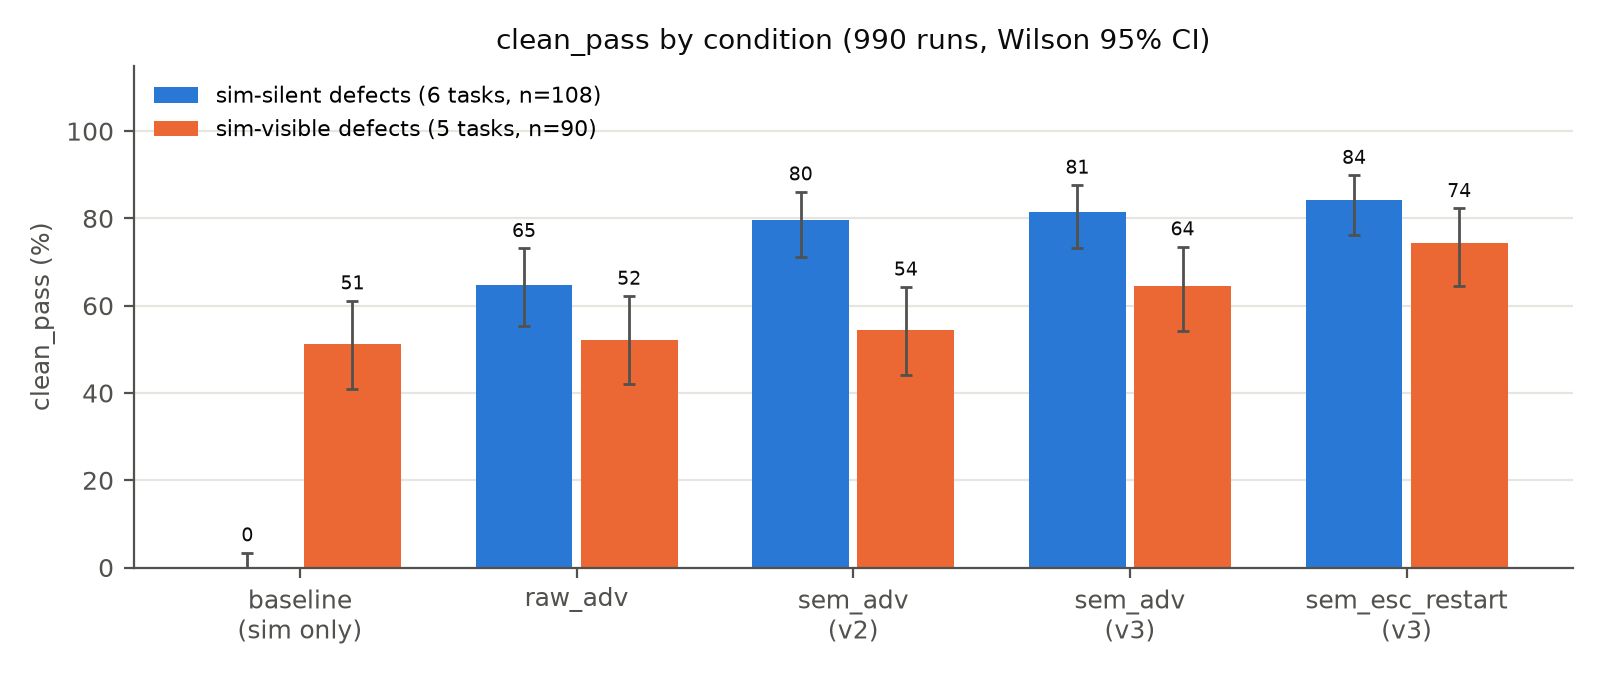
\includegraphics[width=\linewidth]{fig_p3_clean_by_condition.png}
\caption{\texttt{clean\_pass} by condition, split by whether the defect is
visible to simulation. Simulation-only repair scores $0/108$ on sim-silent
defects by construction; every tool condition recovers most of them.}
\label{fig:cond}
\end{figure}

\subsection{Interpretation beats raw tool text, sooner and cheaper}
\label{sec:res-interp}

The cleanest test of the interpreter is \texttt{sem\_adv} against
\texttt{raw\_adv}: the same raw text, the same budget, and directives as the
only difference. v3 reaches $146/198$ against $117/198$, $+14.6$ points with a
cell-level CI of $+3.5$ to $+26.3$ and $43$ discordant pairs in v3's favour
against $14$ (Table~\ref{tab:contrasts}). The gain holds on sim-silent defects
($+16.7$) and points the same way on sim-visible ones ($+12.2$). The
production interpreter already beats raw text ($+9.1$, CI $+1.0$ to $+17.7$),
so the benefit of interpretation predates the upgrade.

\begin{table}[htbp]
\centering
\caption{Paired contrasts on \texttt{clean\_pass} (percentage points),
matched on (model, task, replicate). Cell CI: bootstrap over the $66$
(model, task) cells. Pairs: A-only / B-only discordant pairs, all tasks.}
\label{tab:contrasts}
\small
\begin{tabularx}{\linewidth}{@{} X r c r r r @{}}
\toprule
\textbf{A vs B} & \textbf{$\Delta$ all} & \textbf{cell CI (all)} & \textbf{pairs} & \textbf{$\Delta$ silent} & \textbf{$\Delta$ visible} \\
\midrule
sem\_adv (v3) vs raw\_adv        & $+14.6$ & $[+3.5, +26.3]$   & $43/14$ & $+16.7$ & $+12.2$ \\
sem\_adv (v2) vs raw\_adv        & $+9.1$  & $[+1.0, +17.7]$   & $30/12$ & $+14.8$ & $+2.2$ \\
sem\_esc\_restart vs raw\_adv    & $+20.7$ & $[+11.1, +30.8]$  & $47/6$  & $+19.4$ & $+22.2$ \\
sem\_adv (v3) vs sem\_adv (v2)   & $+5.6$  & $[-2.5, +14.1]$   & $22/11$ & $+1.9$  & $+10.0$ \\
sem\_esc\_restart vs sem\_adv (v3) & $+6.1$ & $[-1.5, +14.1]$  & $21/9$  & $+2.8$  & $+10.0$ \\
\bottomrule
\end{tabularx}
\end{table}

Interpretation is also the cheaper path (Table~\ref{tab:cost}). Against raw
text, v3 uses $0.76$ fewer model calls per run (cell CI $0.20$ to $1.33$) and
$1{,}019$ fewer tokens per run (cell CI $354$ to $1{,}671$), about $23\%$ on
both axes, and spends $4{,}580$ tokens per clean pass against $7{,}440$. It is
faster: $62\%$ of v3 runs are clean after the first model call, against $46\%$
with raw text and $17\%$ with simulation only (Figure~\ref{fig:call}).

\begin{table}[htbp]
\centering
\caption{Cost per condition, $198$ runs each. Tool rounds: model calls whose
prompt carried tool feedback.}
\label{tab:cost}
\small
\begin{tabularx}{\linewidth}{@{} X r r r r r @{}}
\toprule
\textbf{Condition} & \textbf{calls/run} & \textbf{tool rounds/run} & \textbf{tokens/run} & \textbf{calls/clean} & \textbf{tokens/clean} \\
\midrule
baseline               & $1.34$ & $0.00$ & $1{,}425$ & $5.76$ & $6{,}134$ \\
raw\_adv               & $3.27$ & $3.27$ & $4{,}396$ & $5.54$ & $7{,}440$ \\
sem\_adv (v2)          & $2.83$ & $2.83$ & $3{,}831$ & $4.15$ & $5{,}618$ \\
sem\_adv (v3)          & $2.51$ & $2.51$ & $3{,}377$ & $\mathbf{3.40}$ & $\mathbf{4{,}580}$ \\
sem\_esc\_restart (v3) & $2.99$ & $\mathbf{1.32}$ & $3{,}798$ & $3.75$ & $4{,}759$ \\
\bottomrule
\end{tabularx}
\end{table}

\begin{figure}[htbp]
\centering
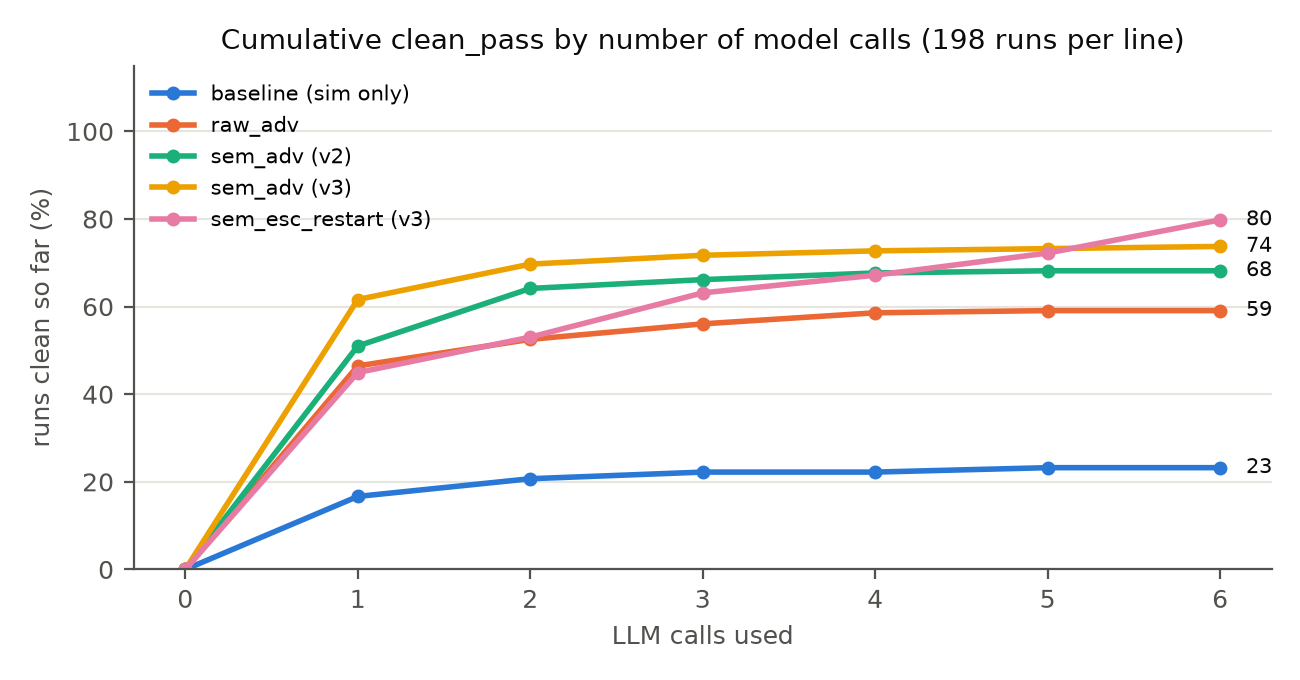
\includegraphics[width=0.85\linewidth]{fig_p3_clean_by_call.png}
\caption{Share of runs clean after each number of model calls. v3 front-loads
its repairs: $62\%$ clean after one call. Escalation, which begins as
baseline, keeps climbing to the highest final rate.}
\label{fig:call}
\end{figure}

\textbf{Across the model ladder.} Interpretation helps most where raw text is
hardest to use (Figure~\ref{fig:models}): v3 minus raw text is $+24.2$ points
on llama3.2:3b, $+18.2$ on gemma3:4b, $+15.2$ on deepseek-coder:6.7b and
$+27.3$ on qwen2.5-coder:7b, which reaches $33/33$ with v3 (the one
per-model gain that survives Holm correction across six models). llama3.1:8b
gains $+3.0$, and qwen2.5-coder:14b is at $33/33$ with any tool feedback, so
there is nothing left to gain.

\begin{figure}[htbp]
\centering
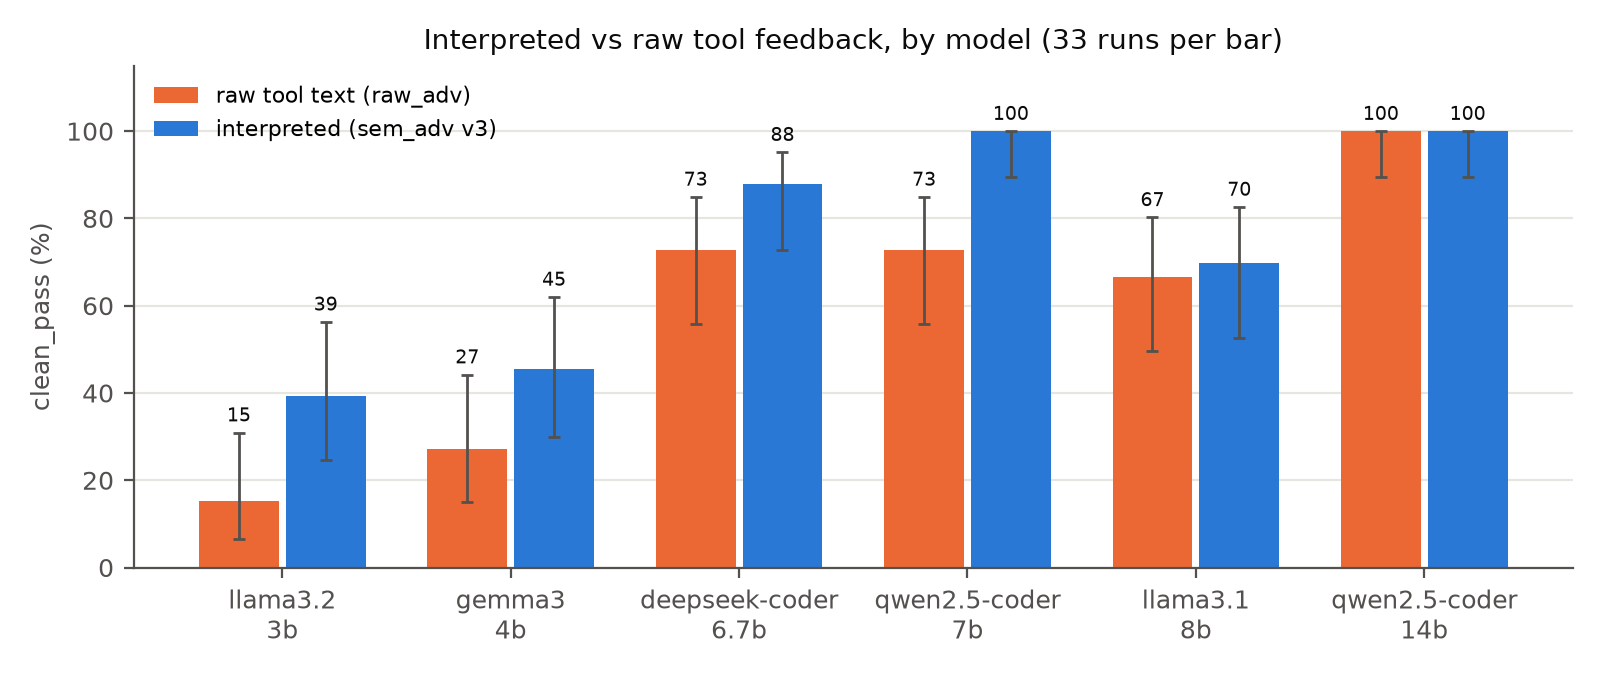
\includegraphics[width=\linewidth]{fig_p3_v3_vs_raw_by_model.png}
\caption{\texttt{clean\_pass} with raw tool text and with v3 directives, per
model ($33$ runs per bar, Wilson $95\%$ CI).}
\label{fig:models}
\end{figure}

\subsection{Per task}
\label{sec:res-task}

Table~\ref{tab:pertask} gives every task. The latch multiplexers are where
interpretation is most decisive: simulation-only repair never touches them,
raw text repairs $60/90$ of the latch tasks, and v3's directives repair
$73/90$ with the interpreter firing in every run. \texttt{MuxPC} and
\texttt{mux3} reach $18/18$ under both interpreters. Two tasks stay at or below half
under every condition: the multi-driven crossbar (\texttt{noc\_xbar4}, at
baseline level, $9$ to $10$ of $18$) and the ALU flags
(\texttt{riscv\_alu\_flags}, at most $9/18$). They mark where the vocabulary
needs to go next.

\begin{table}[htbp]
\centering
\caption{\texttt{clean\_pass} per task, $k/18$ ($6$ models $\times$ $3$
replicates).}
\label{tab:pertask}
\small
\begin{tabularx}{\linewidth}{@{} X c c c c c @{}}
\toprule
\textbf{Task} & \textbf{baseline} & \textbf{raw\_adv} & \textbf{v2} & \textbf{v3} & \textbf{esc (v3)} \\
\midrule
\multicolumn{6}{@{}l}{\emph{Sim-silent}} \\
MuxPC             & $0$  & $17$ & $18$ & $18$ & $18$ \\
execute\_mux      & $0$  & $10$ & $15$ & $15$ & $17$ \\
mem\_wb\_mux      & $0$  & $15$ & $14$ & $13$ & $16$ \\
mux3              & $0$  & $12$ & $18$ & $18$ & $17$ \\
register\_1bit    & $0$  & $10$ & $12$ & $15$ & $16$ \\
riscv\_alu\_flags & $0$  & $6$  & $9$  & $9$  & $7$ \\
\midrule
\multicolumn{6}{@{}l}{\emph{Sim-visible}} \\
Address\_select   & $3$  & $8$  & $9$  & $14$ & $15$ \\
register\_32bit   & $15$ & $11$ & $12$ & $15$ & $16$ \\
register\_4bit    & $14$ & $10$ & $11$ & $14$ & $17$ \\
noc\_xbar4        & $10$ & $9$  & $10$ & $9$  & $9$ \\
ni\_flit\_pack    & $4$  & $9$  & $7$  & $6$  & $10$ \\
\bottomrule
\end{tabularx}
\end{table}

\subsection{The v3 upgrade: the right directive on every task}
\label{sec:res-v3}

Coverage is where the upgrade is unambiguous (Table~\ref{tab:upgrade}). On
\texttt{register\_1bit} and \texttt{ni\_flit\_pack} the production
interpreter produced no directive on the defective input in any of $18$ runs;
v3 fires the intended class in all $18$. On the two latching registers v2
directed the model to gate on the clock; v3 names the missing clock edge. On
\texttt{Address\_select} v2 added a misleading ``gate the output on the
instruction bus'' directive, which v3 suppresses. On the four tasks singled out
before the runs (the two silent and the two misleading ones), clean passes rise
from $42/72$ to $50/72$ ($+11.1$ points, cell CI $-9.7$ to $+31.9$); on
\texttt{register\_1bit} the interpreter-credited wins rise from $3/18$ to
$15/18$. The pass-rate gain is in the favourable direction at this $N$, and
because v3 was written from these designs' logs, the held-out test of the new
rules is a later step.

\begin{table}[htbp]
\centering
\caption{Where production v2 was silent or misleading. Fired: runs in which
the interpreter produced a directive on the defective input ($/18$).
Clean: \texttt{clean\_pass} ($/18$).}
\label{tab:upgrade}
\small
\begin{tabularx}{\linewidth}{@{} l X c c c c @{}}
\toprule
\textbf{Task} & \textbf{v2 on the input} & \textbf{v2 fired} & \textbf{v3 fired} & \textbf{v2 clean} & \textbf{v3 clean} \\
\midrule
register\_1bit  & silent (abort unhandled)          & $0$  & $18$ & $12$ & $15$ \\
ni\_flit\_pack  & silent (expression truncation)    & $0$  & $18$ & $7$  & $6$ \\
register\_32bit & gate on the clock (misleading)    & $18$ & $18$ & $12$ & $15$ \\
register\_4bit  & gate on the clock (misleading)    & $18$ & $18$ & $11$ & $14$ \\
Address\_select & extra gating directive on a bus   & $18$ & $18$ & $9$  & $14$ \\
\bottomrule
\end{tabularx}
\end{table}

\subsection{Escalation: highest clean rate, fewest tool rounds}
\label{sec:res-esc}

Escalation reaches the highest \texttt{clean\_pass} ($158/198$, $80\%$) and
matches baseline's $85\%$ simulation pass rate, with $1.32$ tool-feedback
rounds per run against $2.51$ for always-on v3 ($47.5\%$ fewer). On the
sim-visible tasks, where simulation-only repair does run the model, escalation
beats it by $+23.3$ points ($67/90$ against $46/90$, cell CI $+8.9$ to
$+37.8$), and on deepseek-coder:6.7b and qwen2.5-coder:7b it reaches $15/15$
there against baseline's $9/15$. It also protects the smallest model: on
sim-visible tasks llama3.2:3b is at $9/15$ with simulation only and $1/15$ with
raw text every round, and escalation holds it at $8/15$. $109$ runs never
needed to escalate ($105$ of them ended clean); the $89$ that did ended $53$
clean.

\subsection{Repaired leaves restore the real designs}
\label{sec:res-compose}

Each (model, replicate) set of final leaves was spliced back into the real
designs and re-synthesised (Table~\ref{tab:compose},
Figure~\ref{fig:compose}). Simulation-only repair never yields a synthesisable
design ($0/18$ in each), because it never touches the sim-silent register
that aborts synthesis. v3 restores top-level synthesis in $16/18$ groups for
each design; escalation in $18/18$ for both meshes. Leaf-level
\texttt{clean\_pass} was sufficient for composition in every case: whenever
all composed leaves were clean, the design reached the golden bound of
Table~\ref{tab:prop} ($32/32$ for each mesh, $27/27$ for the MPSoC).

\begin{table}[htbp]
\centering
\caption{Top-level synthesis pass after splicing in each condition's repaired
leaves ($18$ model $\times$ replicate groups per cell), and in brackets the
groups that also reach the golden latch bound. Synthesis only.}
\label{tab:compose}
\small
\begin{tabularx}{\linewidth}{@{} X c c c c c @{}}
\toprule
\textbf{Design} & \textbf{baseline} & \textbf{raw\_adv} & \textbf{v2} & \textbf{v3} & \textbf{esc (v3)} \\
\midrule
$2{\times}2$ mesh & $0$ ($0$) & $15$ ($10$) & $13$ ($11$) & $16$ ($15$) & $\mathbf{18}$ ($\mathbf{16}$) \\
$3{\times}3$ mesh & $0$ ($0$) & $15$ ($10$) & $13$ ($11$) & $16$ ($15$) & $\mathbf{18}$ ($\mathbf{16}$) \\
MPSoC top         & $0$ ($0$) & $13$ ($8$)  & $12$ ($8$)  & $\mathbf{16}$ ($\mathbf{14}$) & $15$ ($13$) \\
\bottomrule
\end{tabularx}
\end{table}

\begin{figure}[htbp]
\centering
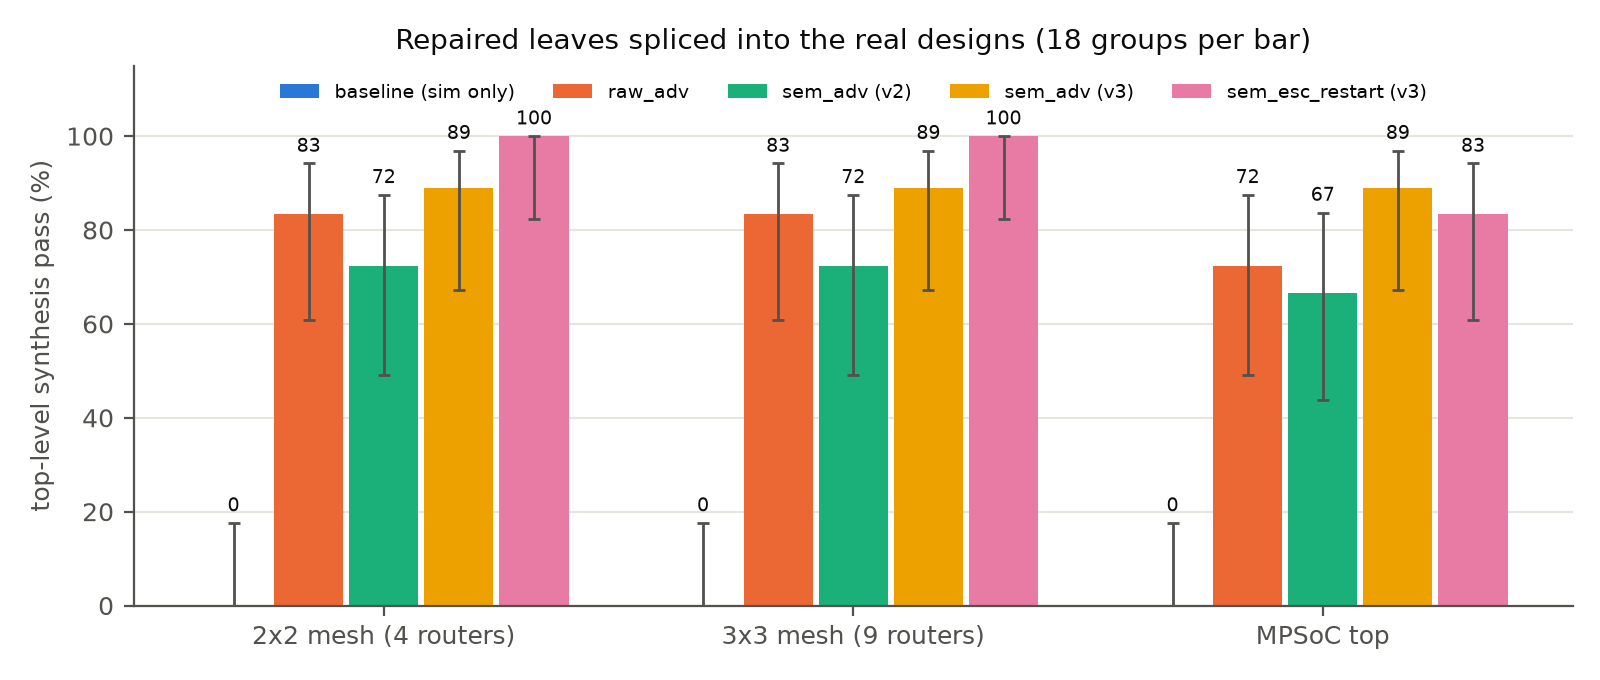
\includegraphics[width=\linewidth]{fig_p3_composition.png}
\caption{Top-level synthesis pass of the two meshes and the MPSoC after
splicing in repaired leaves, by condition (Wilson $95\%$ CI).}
\label{fig:compose}
\end{figure}

% ============================================================================
\section{What Phase 3 Establishes, and What the Next Runs Address}
\label{sec:summary}

On real multiprocessor RTL the question is not whether a module simulates but
whether the design can be signed off. There, a simulation-only loop is
structurally blind: it signed off every simulation-silent defect in this
study. The synthesis and lint layer makes those defects visible, and the
interpreter turns visibility into repairs more reliably, sooner and more
cheaply than raw tool text. Leaf repairs compose: a handful of repaired
definitions restores synthesis of networks with $4$ and $9$ routers and of
the processor top. And the interpreter can keep up with new designs: real logs
exposed missing vocabulary, and an additive, regression-gated layer closed it
without disturbing earlier results.

The next runs sharpen four points:
\begin{enumerate}[leftmargin=1.2em, itemsep=0.1em]
\item \textbf{Held-out defects} for the v3 rules, which were written from
these designs' logs.
\item \textbf{A control arm} that gives baseline escalation's generic
sign-off message without any tool detail, to separate being told that sign-off
failed from being told what failed.
\item \textbf{Keeping the best candidate.} Some runs pass simulation at some
point (the defective input included) and lose it later ($23$ of $198$ under v3, $11$ under
escalation); returning the best candidate so far would recover them.
\item \textbf{More replicates} on the tasks that stayed flat
(\texttt{noc\_xbar4}, \texttt{riscv\_alu\_flags}), where the replicate
correlation leaves per-task comparisons with little power, and
integration-level feedback for defects that only exist once modules are
connected (a one-bit program-counter port driven with $32$ bits, a FIFO
instantiated positionally with a missing port).
\end{enumerate}

\end{document}
